\documentclass[a4paper, 12pt]{article}

\usepackage{amsmath}
\usepackage{array}
\usepackage{hyperref}
\usepackage{cleveref}
\hypersetup{
	colorlinks=true,
	linkcolor=blue,
	filecolor=blue,
	citecolor = black,
	urlcolor=cyan,
}

\usepackage{graphicx}
\usepackage{caption}
\usepackage[section]{placeins}
\usepackage{lipsum}


%for code(MATLAB in particular)
\usepackage{listings}
\usepackage{color} %red, green, blue, yellow, cyan, magenta, black, white
\definecolor{mygreen}{RGB}{28,172,0} % color values Red, Green, Blue
\definecolor{mylilas}{RGB}{170,55,241}

\lstset{
    language=Matlab,%
    %basicstyle=\color{red},
    breaklines=true,%
    morekeywords={matlab2tikz},
    keywordstyle=\color{blue},%
    morekeywords=[2]{1}, 
    keywordstyle=[2]{\color{black}},
    identifierstyle=\color{black},%
    stringstyle=\color{mylilas},
    commentstyle=\color{mygreen},%
    showstringspaces=false,%without this there will be a symbol in the places where there is a space
    numbers=left,%
    numberstyle={\tiny \color{black}},% size of the numbers
    numbersep=7pt, % this defines how far the numbers are from the text
    emph=[1]{for,end,break},
    emphstyle=[1]\color{red}, %some words to emphasise
    %emph=[2]{word1,word2}, emphstyle=[2]{style},
}


\graphicspath{{./pictures/}}

\title{ECEN315 - Assignment 2}
\author{Joshua Benfell - 300433229}

\begin{document}
    \maketitle

    \section{Question 1}
        \lstinputlisting{../q1.m}
        
        \begin{table}[!h]
            \caption{Time Constants and Settling Time for Various Step Inputs}
            \label{tab:q1}
            \centering
            \begin{tabular}{r|c|r}
                Step Size & Time Constants & Settling Time\\
                \hline
                1 & $\sqrt{3.7321 \times 0.2679} = 0.9999$ & 14.879\\
                2 & $\sqrt{1.7071 \times 0.2929} = 0.7071$ & 6.9996\\
                4 & $\sqrt{0.5 \times 0.5} = 0.5$ & 2.1970\\
                8 & $\sqrt{0.5 \times 0.5} = 0.5$ & 2.1082

            \end{tabular}
        \end{table}

        \begin{figure}[!h]
            \centering
            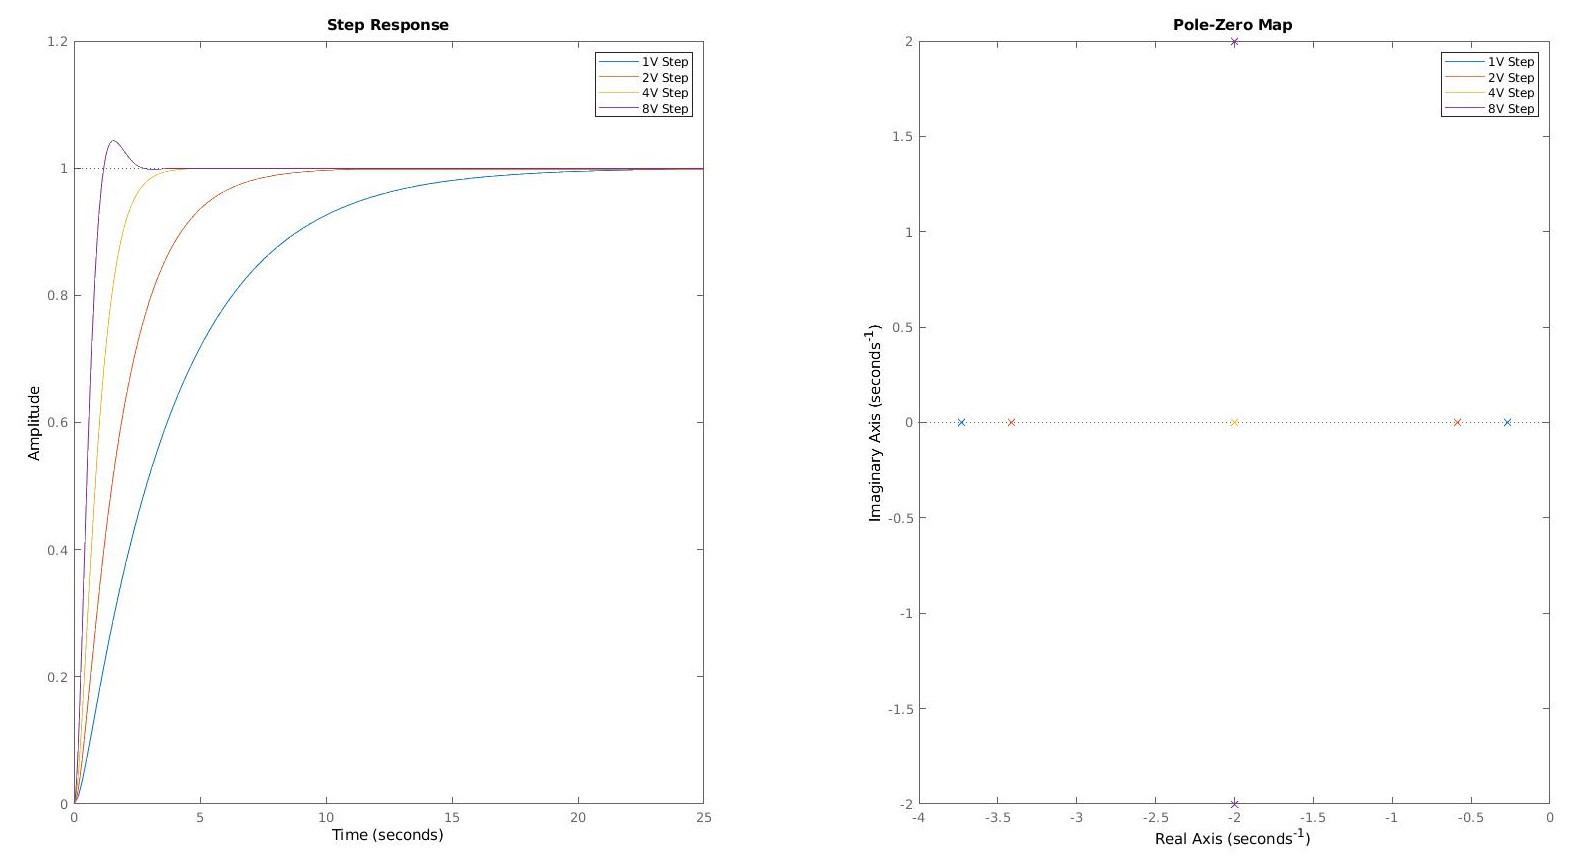
\includegraphics[width=\textwidth]{q1.jpg}
            \caption{Step Response to various step sizes and PZ Map of those step responses}
            \label{fig:q1}
        \end{figure}


        By changing the value of a, the transfer function goes from over to underdamped. a values of 1 and 2 make the system over damped, 4 is critically damped and 8 makes it under damped, reflected by the overshoot. We can confirm the nature of the step responses by looking at the poles. When a is 1 or 2, the poles are real and negative but not the same, so we know that it's over damped. When a is 4, the poles are negative and equal, so it's critcally damped. Finally when a is 8, the poles are complex which introduces oscillatory factors to the response, and therefore the system is underdamped.   
        \par
        From the settling times we can see that the higher a is the faster the response settles. This makes sense as critically damped is the fastest that it can settle without oscillation, whereas over damped systems go slower and under damped systems are faster at rising, but if there's too much oscillation it will take a while to settle. Because there's small oscillation, it makes sense to settle faster than the critically dameped system.
        \par
        There appears to be two time constants for the over damped systems and 1 for the critically damped and under damped systems. By square rooting the product we can get a time constant for the system. The more damping on a system indicates multiple first order systems acting on it. Overdamped systems have two poles where one is dominant shown by the longer time constant and the other is not, meaning we could simplify the system to be first order. Critically damped systems having two time constants the same makes sense as the poles are in the same place, same goes for the underdamped system as those poles are complex conjugates. The lower the time constant seems to indicate a faster response, and it can be seen that the critical and under damped system settle in about the same time.

    \section{Question 2}

        \lstinputlisting{../q2.m}

        \begin{figure}[!h]
            \centering
            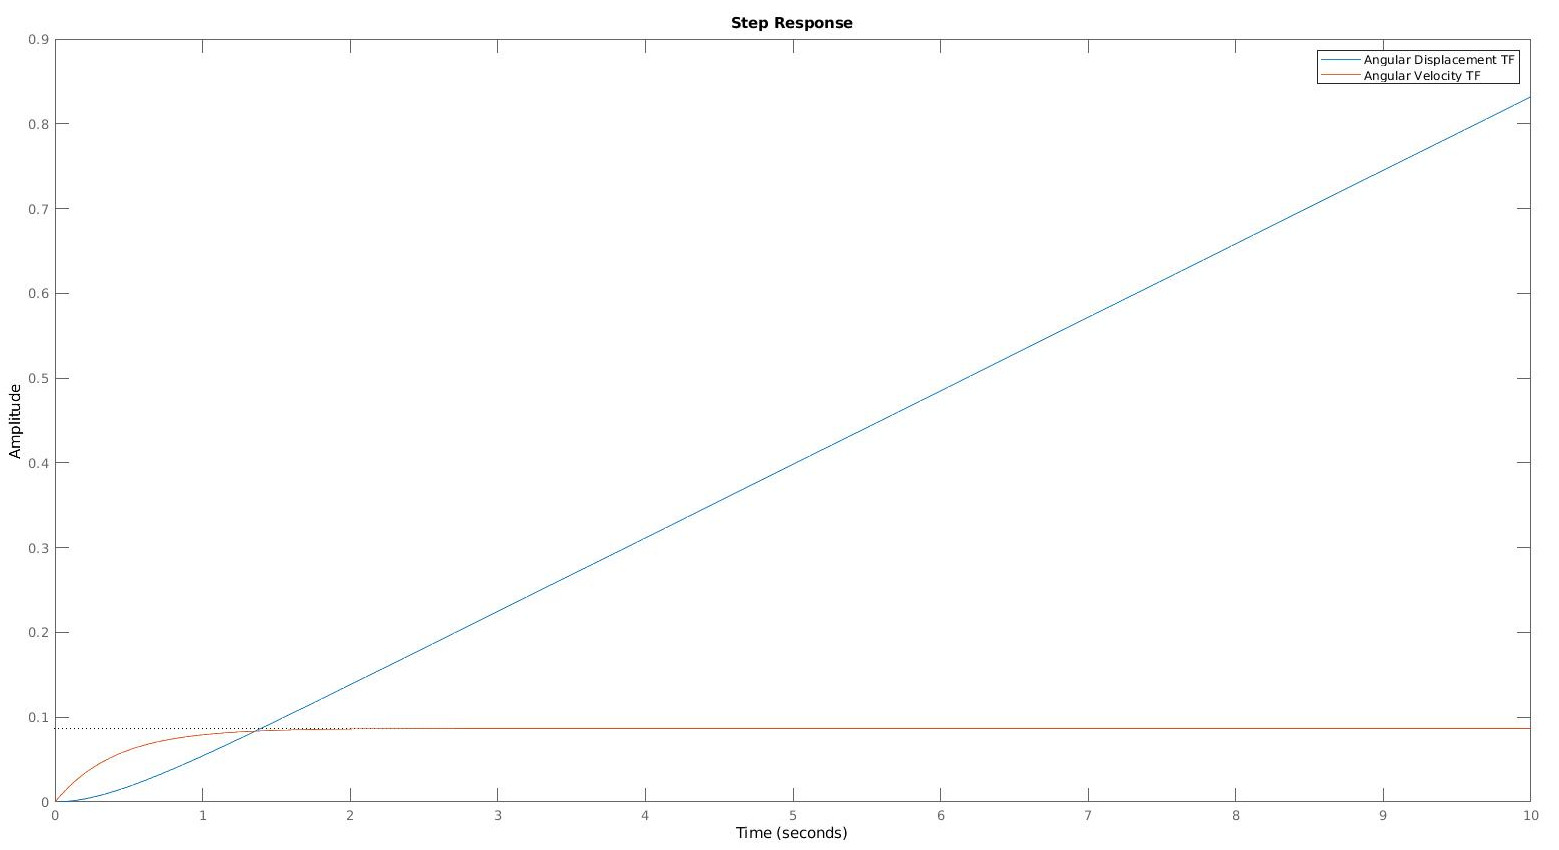
\includegraphics[width=\textwidth]{q2.jpg}
            \caption{Step Response of $\frac{\Theta_L(s)}{E_a(s)}$ and $\frac{\Omega_L(s)}{E_a(s)}$}
            \label{fig:q2}
        \end{figure}

        The blue line in \cref{fig:q2} is the response for the transfer function in a. This transfer function just continues with a positive gradient after a step response is added. This makes sense as it is a motor, so unless you wrap around once you hit $2\pi$ radians, the displacement will technically always increase.
        \par
        This is reflected in part b. When we want to get the angular velocity over the applied voltage, we differentiate the function. To do this in the frequency domain, we multiply by s. This results in the following transfer function:
        \begin{equation}
            \frac{\Omega_L(s)}{E_a(s)} = \frac{0.0425}{s+2.45}
        \end{equation}
        This is a first order transfer functon that has a steady state of $0.01735 * E_a$. For a 5V step, this is a steady state gain of $0.0867 rads/sec$ which is how much the motor shaft spins every second.

    \section{Question 3}

        \lstinputlisting{../q3.m}
        \begin{table}[!h]
            \centering
            \caption{Relevant values for the systems defined in question 3}
            \label{tab:q3}
            \begin{tabular}{l|r|r|r|r|r|r}
                System & $\omega_n$ & $\zeta$ & $T_s$ (s) & $T_p$ (s) & $T_R$ (s) & $OS\%$ \\ 
                \hline
                $G_1(s)$ & $4$   & $0.375$ & $2.66$ & $0.86$ & $0.357$ & $28$ \\
                $G_2(s)$ & $0.2$ & $0.05$  & $3.8$  & $15.7$ & $5.42$  & $85.4$ \\
                $G_3(s)$ & $3.2711 \times 10^3$ & $0.2446$ & $0.00433$ & $0.000979$ & $0.0003864$ & $45.2$
                
            \end{tabular}
        \end{table}

        \begin{figure}[!h]
            \centering
            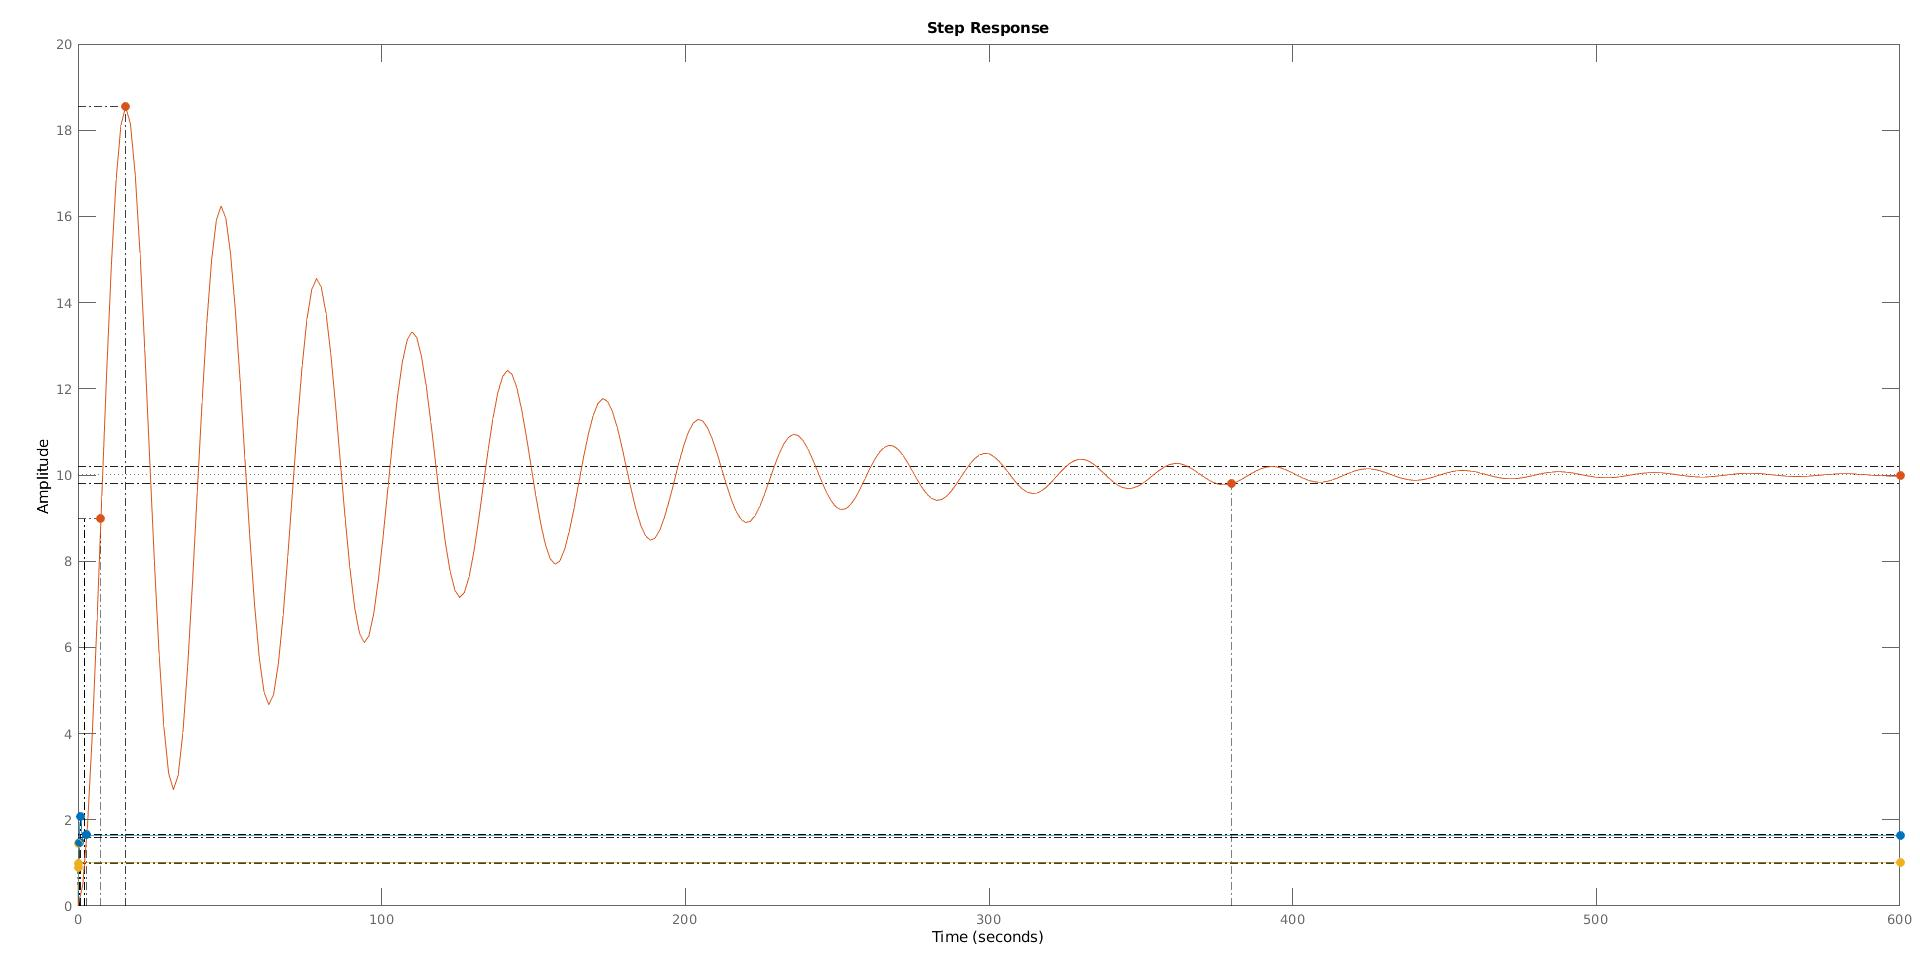
\includegraphics[width=\textwidth]{q3.jpg}
            \caption{Usage of the LTI Viewer exported to figure}
            \label{fig:q3}
        \end{figure}

        In \cref{fig:q3} the systems are assigned as follows, $G_1$ is blue, $G_2$ is Orange, $G_3$ is yellow (light brown). All systems are under damped but, $G_1$ and $G_3$ are the lest under damped, the overshoot the target a little bit and settle quickly. $G_2$ is severly under damped, it oscillates quite a lot before settling. 

    \section{Question 4}

        \lstinputlisting{../q4.m}

        \begin{figure}[!h]
            \centering
            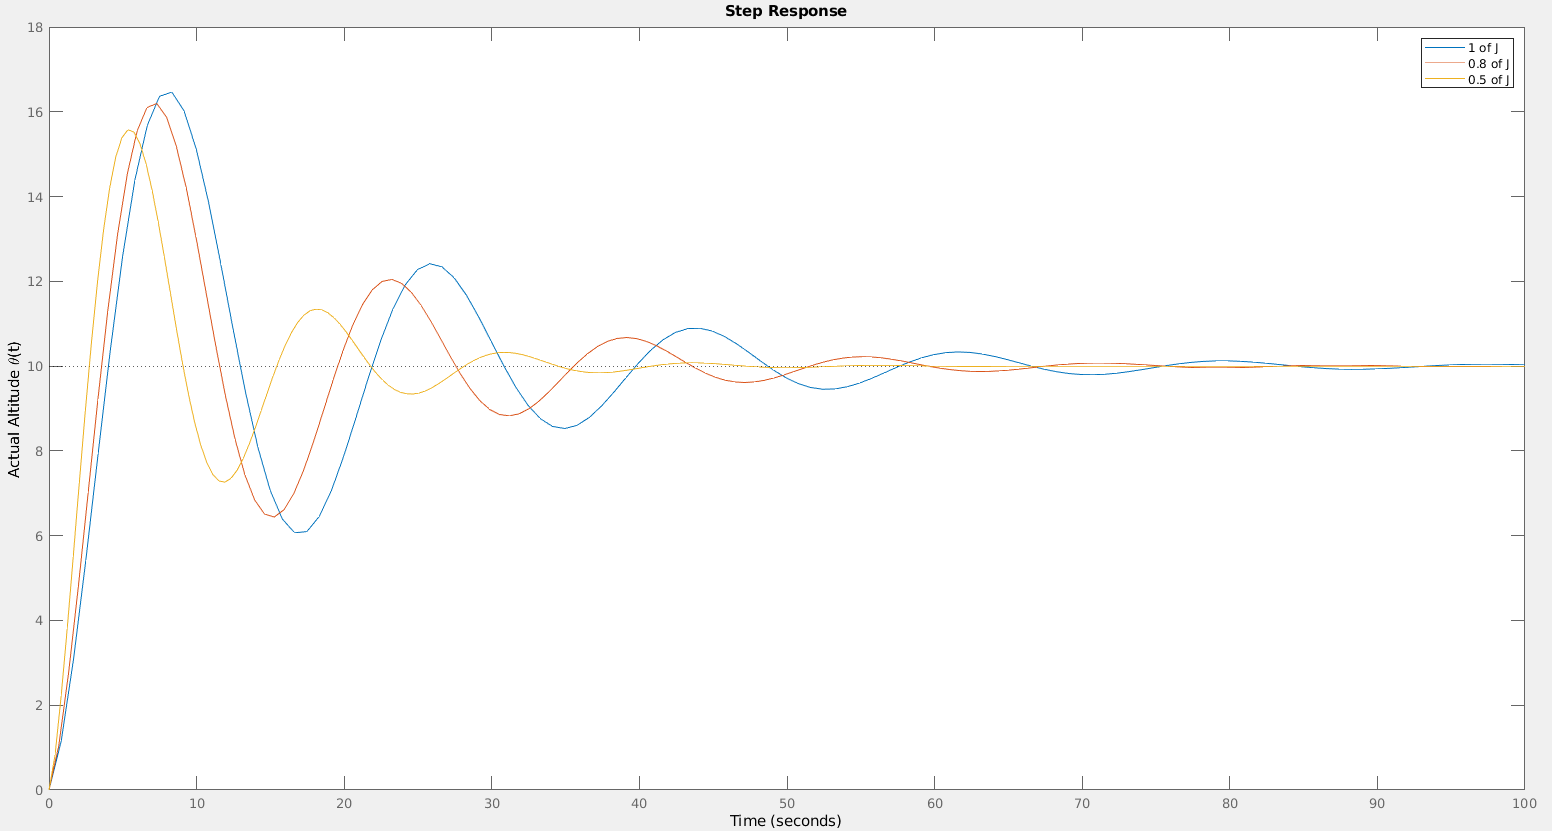
\includegraphics[width=\textwidth]{q4.png}
            \caption{Satellite Step Responses for various moments of inertia}
            \label{fig:q4}
        \end{figure}

        As seen in \cref{fig:q4} the decrease in J causes a faster transient response and smaller overshoot which means faster settling. This is because the Satellite doesn't have enough damping. Any push in a direction may overshoot the target and requires a push in the other direction to keep heading towards it. When the Satellite has a higher moment of inertia it resists the angular change and torque more so requires more torque to slow down and move in the other direction. Which is why we see larger amplitudes for higher J. With lower J, it takes less time to slow, stop and start the Satellite turning.

    \section{Question 5 (6 in the handout)}

        \lstinputlisting{../q6.m}

        \begin{figure}[!h]
            \centering
            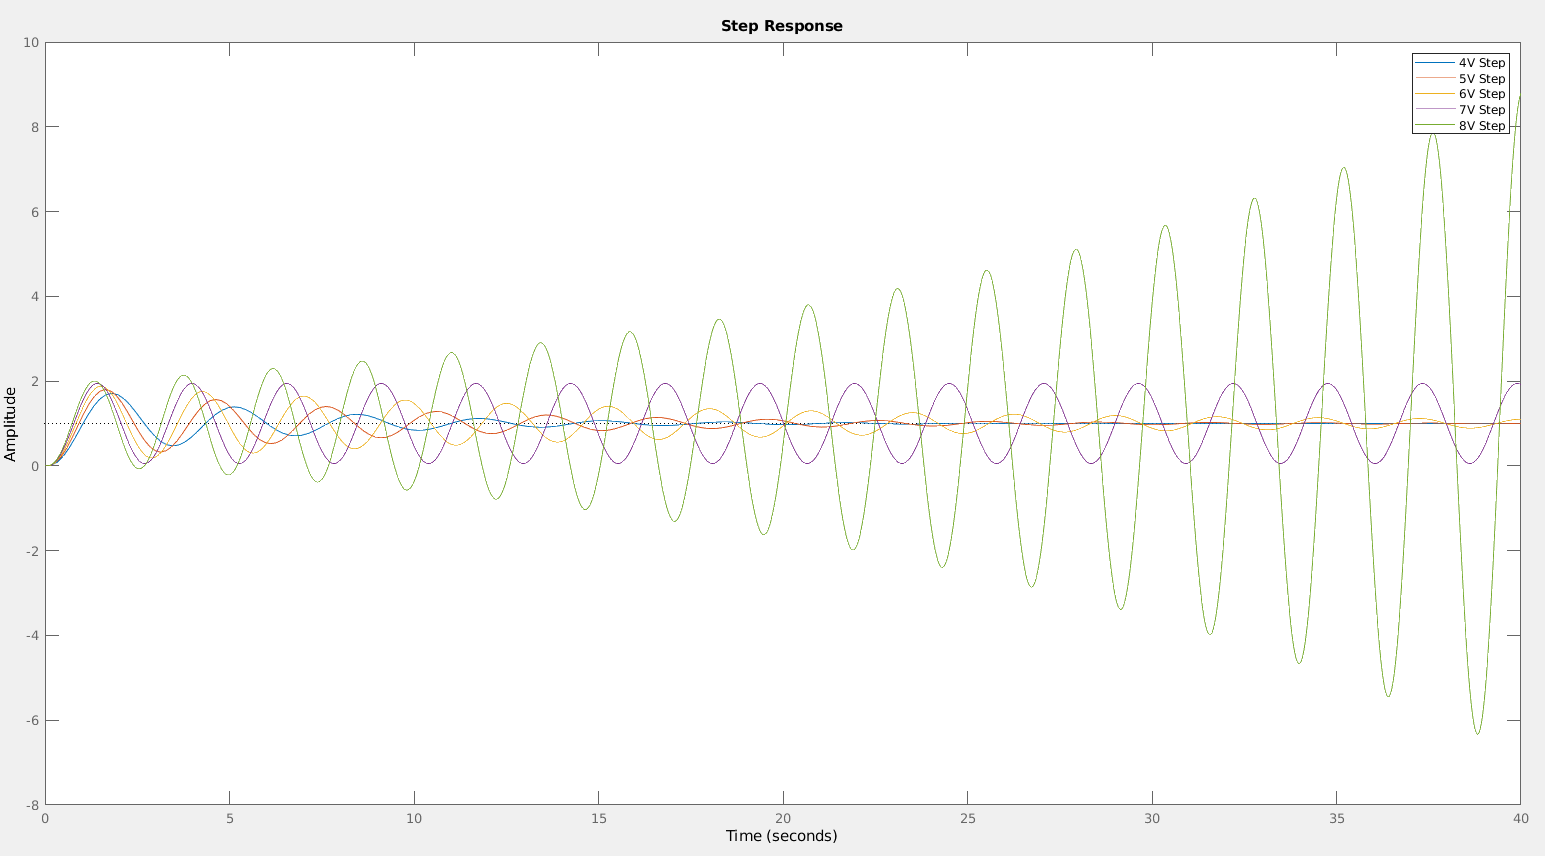
\includegraphics[width=\textwidth]{q5.png}
            \caption{Gain Controller Step Response Stability}
            \label{fig:q5a}
        \end{figure}

        \begin{figure}[!h]
            \centering
            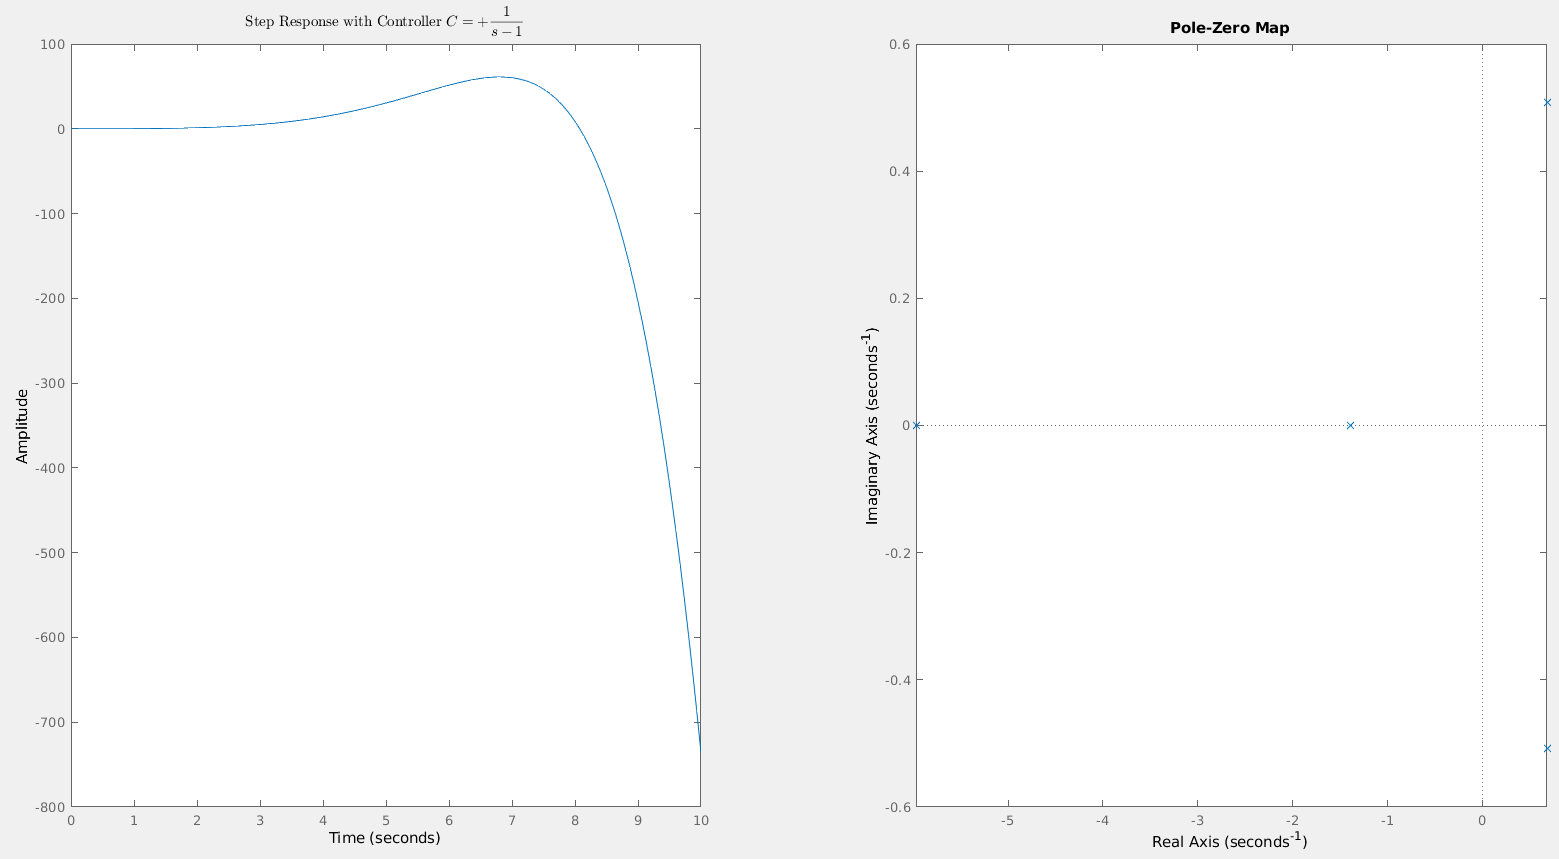
\includegraphics[width=\textwidth]{q5b.png}
            \caption{PI Controller Stability with low steady state gain}
            \label{fig:q5b}
        \end{figure}

        For the first part of this question, we can see in \cref{fig:q5a} that a gain controller of 7 provides no damping on the system. This indicates that anything higher than 7 will make the system unstable and this is the maximum value that can be used for stability.
        \par
        For the second part of this question we can use a controller that introduces a pole with a positive real component. Doing this will make it unstable. Here I am using $C = \frac{1}{s-1}$, which has a steady state gain of 1.
        

\end{document}